\section{Algorytm Rabina-Karpa}
\subsection{Opis}
Jest to algorytm przeszukiwania tekstu zaproponowany przez \textit{Richarda Karpa oraz Michaela Rabina} i przedstawiony światu w 1987 roku na łamach magazynu \textit{IBM Journal of Research and Development} w artykule \textit{Efficient randomized pattern-matching algorithms} \cite{rabin_karp_alg}.\\
Algorytm \say{naiwny} dla tego problemu oparty jest na porównywaniu szukanego wzorca z każdą pozycją w tekście, co w najgorszym przypadku cechuje się złożonością obliczeniową \textit{O(n*m)} (gdzie \textit{n} to długość szukanego wzorca, a \textit{m} to długość przeszukiwanego tekstu).
Alogrytm \textit{Rabina-Karpa} stanowi usprawnienie \say{naiwnego} podejścia poprzez wykorzystanie:
\begin{itemize}
    \item elementarnego pojęcia teorii liczb jakim jest przystawanie dwóch liczb modulo,
    \item funkcji haszującej \textit{$h(x_{i})$},
    \item funkcji obliczającej \say{kroczący} hasz (ang. \textit{rolling hash}) niskim kosztem  poprzez wyznaczenie \textit{$h(x_{i+1})$} na podstawie \textit{$h(x_{i})$}.
\end{itemize}
Kluczowa, dla algorytmu, jest interpretacja alfabetu $\sum$, która pozwala traktować tekst \textit{k} symboli jako liczbę \textit{k-cyfrową} w systemie o podstawie \textit{d} (gdzie \textit{$d = |\sum|$}). Interpretacja ta odbywa się za pomocą wyliczania wartości hasza dla zadanego podciągu przeszukiwanego tekstu. Wartość hasza obliczana jest za pomocą reguły \textit{Hornera}:
\[ hasz = wzorzec[n-1] + d(wzorzec[n-2] + d(wzorzec[n-3]) + \ldots + d(wzorzec[1] + d*wzorzec[0]) \ldots ))\]
W celu zapewnienia stałego czasu wykonywania operacji arytmetycznych podczas wyliczania wartości hasza dla dowolnie długich podciągów, stosuje się dzielenie modulo \textit{q}. Powszechną praktyką jest, aby wybrana liczba \textit{q} była liczbą pierwszą oraz aby wartość \textit{d*q} mieściła się w zakresie słowa maszynowego procesora, co zapewnia wykonanie wszystkich operacji arytmetycznych z pojedynczą precyzją.
Proces obliczania wartości \say{kroczącego} hasza został przedstawiony na rysunku \ref{fig:rolling_hash}.
\begin{figure}[H]
    \centering
    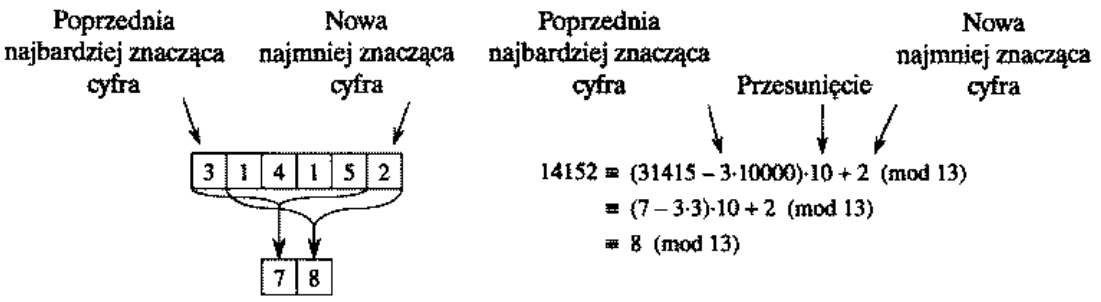
\includegraphics[width=\linewidth]{images/RollingHash.png}
    \caption{Schemat obliczania wartości \glqq kroczącego\grqq \space hasza \cite{cormen}}
    \label{fig:rolling_hash}
\end{figure}
Mając obliczone wartości funkcji haszującej dla wzorca i wybranego podzbioru tesktu możemy sprawdzić, czy następuje wystąpienie wzorca w tekście. Warto zaznaczyć, że samo porównanie wartości haszów nie wystarcza; kongruentność dwóch liczb nie implikuje ich równości. Jeżeli wartości haszy są sobie równe należy sprawdzić, czy wybrany pozdbiór tesktu i wzorzec to te same słowa. Natomiast, jeżeli wartości haszy nie są sobie równe należy zacząć liczenie \say{kroczącego} hasza dla następnej pozycji; jeżeli dwie liczby nie przystają do siebie modulo to na pewno nie są sobie równe.
\subsection{Cechy}
Algorytm cechuje się oczekiwaną złożonością czasową \textit{O(m+n)} oraz pesymistyczną złożonością czasową \textit{$O((m-n + 1)n) \approx O(m*n)$}. W implementacji algorytmu można podzielić szukany tekst na mniejsze fragmenty przy jednoczesnym zachowaniu założeń proponowanej metody (operacja fragmentaryzacji tekstu nie jest obarczona dużą złożonością czasową). Pomimo swojej sekwencyjnej natury, algorytm daje się w łatwy sposób zrównoleglić. 